\documentclass[a4paper,12pt]{article}
\usepackage[utf8]{inputenc}
\usepackage{polski}
\usepackage{tgtermes}
\usepackage{geometry}
\geometry{left=2.5cm, right=2.5cm, top=2.5cm, bottom=2.5cm}
\usepackage{graphicx}
\usepackage{ragged2e}
\usepackage{array}
\usepackage{mathtools,amsthm,amssymb,icomma,upgreek,xfrac}
\usepackage{bm}
%\usepackage{minted}
\mathtoolsset{showonlyrefs,mathic}
\usepackage{tikz}
\usetikzlibrary{quotes,angles}
\usepackage{circuitikz}
\usepackage{titlesec} % Pakiet do modyfikacji sekcji
\usepackage{enumitem}
\usepackage{float}
\usepackage{hyperref}
\hypersetup{colorlinks=true,linkcolor=blue,urlcolor=blue}



\title{Sprawozdanie: Analiza porównawcza danych rzeczywistych z wykorzystaniem metod statystyki opisowej}
\date{\today}

\begin{document}
	\maketitle
	
	{\small \section{Wstęp}}
	Wybrany przez nas zbiór danych pochodzi ze strony podanej na liście 2   i jest zatytułowany \href{https://vincentarelbundock.github.io/Rdatasets/doc/AER/Guns.html}{"More Guns, Less Crime?"}. Zawiera on informacje zebrane w latach 1977-1999 w 51 stanach USA (dodany District of Columbia) o użyciu broni, liczbie przestępstw, wybrane informacje o ludności i tym czy w danym roku stan miał "shall carry law". Shall carry law jest przepisem dotyczącym noszenia broni palnej. To prawo zobowiązuje urzędników do wydania pozwolenia na ukryte noszenie broni palnej, jeżeli osoba spełnia pewne określone kryteria. Celem naszej analizy będzie porównanie statystycznych cech przestępczości w stanach z i bez tego prawa. Zmienne z tego zbioru danych, na których będziemy się skupiać to
	\begin{itemize}[itemsep=5pt,parsep=0pt]
			\item law -- przyjmuje wartości "yes" i "no", mówi o tym czy w danym roku i stanie obowiązywało prawo dotyczące noszenia broni palnej,
			\item violent -- wskaźnik przestępczości z użyciem przemocy (liczba incydentów na $100000$ mieszkańców).
	\end{itemize}
	
	{\small \section{Analiza rozkładu przy pomocy metryk statystycznych}} 
	\subsection{Miary położenia}
	
	1. Średnią arytmetyczną dla próby $x_1, x_2, ..., x_n$ obliczamy wykorzystując następujący wzór
	\begin{equation}
		\bar x = \frac{1}{n} \sum_{i=1}^{n} x_i.
	\end{equation}
	Średnia dla danych
	\begin{itemize}[itemsep=5pt,parsep=0pt]
		\item z prawem (data['law'] == 'yes') wynosi 381.05087719298245,
		\item bez prawa (data['law'] == 'no') 542.2377252252252.
	\end{itemize}
	Widzimy zatem, że w stanach i latach, kiedy noszenie ukrytej broni palnej było regulowane, ilość przestępstw z użyciem przemocy była mniejsza o około 161 przypadków na 100 000 mieszkańców. Możemy z tego wywnioskować, że uregulowanie i nałożenie przepisów na osoby noszące broń palną zmniejsza znacząco ilość przemocowych przestępstw. \\
	
	\noindent 2. Mediana, inaczej drugi kwartyl (Q2), jest miarą położenia, która wyznacza miejsce, gdzie w szeregu uporządkowanym, powyżej i poniżej znajduje się taka sama liczba obserwacji. 
	\begin{equation}
		x_{\text{med}} = \left\{ 
		\begin{array}{ll}
			x_{(n+1)/2}, & \text{dla $n$ nieparzystego} \\
			\frac{1}{2}(x_{n/2} + x_{1 + n/2}), & \text{dla $n$ parzystego}
		\end{array}
		\right.
	\end{equation}
	Mediana dla danych
	\begin{itemize}[itemsep=3pt,parsep=0pt]
		\item z prawem wynosi 322.0,
		\item bez prawa 478.4.
	\end{itemize}
	Wartość środkowa liczby przestępstw jest wyraźnie niższa w grupie z obowiązującym prawem dotyczącym broni. Oznacza to, że typowy poziom przemocy (czyli taki, którego nie zaburzały wartości skrajnie wysokie lub niskie) był znacznie niższy w stanach, które miały takie regulacje. Mediana jest szczególnie odporna na wartości odstające, dlatego wynik ten dodatkowo potwierdza, że ogólny poziom przemocy był w tych stanach niższy --- nawet jeśli zdarzały się przypadki wyjątkowo wysokie. \\
	
	\noindent 3. Kwartyle (Q1, Q3) - pierwszy kwartyl (Q1) to mediana grupy obserwacji mniejszych od Q2 (mediany całego zbioru danych), a trzeci kwartyl (Q3) to mediana grupy obserwacji większych od Q2.
	Kwartyle dla danych
	\begin{itemize}[itemsep=5pt,parsep=0pt]
		\item z prawem wynoszą Q1 = 149.5, Q3 = 514.6,
		\item bez prawa Q1 = 315.0, Q3 = 676.4.
	\end{itemize}
	Wartości kwartylowe pozwalają określić, jak dane są rozłożone i gdzie znajduje się większość obserwacji. Widzimy, że zarówno pierwszy (Q1), jak i trzeci kwartyl (Q3) są znacznie niższe w grupie z obowiązującym prawem dotyczącym broni. Oznacza to, że $75\%$ przypadków przemocy w tej grupie nie przekracza poziomu 514,6, podczas gdy w grupie bez prawa aż $75\%$ obserwacji mieści się dopiero poniżej 676,4. Świadczy to o niższym ogólnym poziomie przemocy w stanach z regulacją prawną. \\
	
	\subsection{Miary zmienności (rozproszenia)}
	1. Rozstęp dla próby (danych) uporządkowanych $x_1, x_2, ..., x_n$ obliczamy
	\begin{equation}
		\text{R} = x_n - x_1
	\end{equation}
	Rozstęp dla danych
	\begin{itemize}[itemsep=5pt,parsep=0pt]
		\item z prawem wynosi 1193.0,
		\item bez prawa 2874.8.
	\end{itemize}
	Rozstęp informuje o zakresie zmienności danych. Dla stanów bez prawa rozstęp jest ponad dwa razy większy, co oznacza dużo większe zróżnicowanie liczby przestępstw z użyciem przemocy w tej grupie. To może sugerować, że brak regulacji prowadzi do mniej stabilnych i bardziej nieprzewidywalnych wyników. \\
	
	\noindent 2. Rozstęp międzykwartylowy (IQR)
	\begin{equation}
		\text{IQR} = \text{Q3} - \text{Q1}
	\end{equation}
	Rozstęp międzykwartylowy dla danych
	\begin{itemize}[itemsep=5pt,parsep=0pt]
		\item z prawem wynosi 365.1,
		\item bez prawa 361.4.
	\end{itemize}
	Mimo że wartości IQR są do siebie zbliżone w obu grupach, nieco większy rozstęp w stanach z prawem może wskazywać, że środkowa połowa danych jest tam bardziej rozciągnięta, choć ogólna przemoc w tej grupie jest niższa. To może sugerować większą różnorodność w umiarkowanym zakresie przestępczości, ale niekoniecznie przypadki ekstremalne. \\
	
	\noindent 3. Wariancja
	\begin{equation}
		\text{Var}X = \mathbb{E}(X - \mathbb{E}X)^2 = \frac{1}{n} \sum_{i=1}^{n} (x_i - \bar x)^2.
	\end{equation}
	Wariancja dla danych
	\begin{itemize}[itemsep=5pt,parsep=0pt]
		\item z prawem wynosi 70801.25821852878,
		\item bez prawa 118442.36169617675.
	\end{itemize}
	
	\noindent 4. Odchylenie standardowe (obciążone, czyli dzielimy przez $n$ a nie $n-1$)
	\begin{equation}
		\text{S} = \sqrt{\frac{1}{n} \sum_{i=1}^{n} (x_i - \bar x)^2}.
	\end{equation}
	Odchylenie standardowe dla danych
	\begin{itemize}[itemsep=5pt,parsep=0pt]
		\item z prawem wynosi 266.0850582398959,
		\item bez prawa 344.15456076620103.
	\end{itemize}
	Wariancja i odchylenie standardowe są istotnie wyższe w grupie bez prawa, co potwierdza, że rozrzut danych (czyli odchylenia od średniej) jest znacznie większy. Świadczy to o tym, że przemoc w tych stanach występuje z dużo większym natężeniem i zróżnicowaniem. \\
	
	\noindent 5. Współczynnik zmienności
	\begin{equation}
		\text{V} = \frac{\text{S}}{\bar x} \cdot 100\%
	\end{equation}
	Współczynnik zmienności dla danych
	\begin{itemize}[itemsep=5pt,parsep=0pt]
		\item z prawem wynosi 69.82927324561378$\%$,
		\item bez prawa 63.46931332069382$\%$.
	\end{itemize}
	Współczynnik zmienności pozwala porównać zmienność względną, czyli jak bardzo dane są rozproszone względem swojej średniej. Ciekawym wynikiem jest to, że grupa z prawem ma wyższy współczynnik zmienności, co oznacza, że przy niższej średniej przestępczości dane są bardziej rozproszone względem tej średniej. Warto jednak zauważyć, że różnica nie jest duża, a ogólny poziom przemocy i tak pozostaje niższy w tej grupie. \\
	
	\subsection{Miary kształtu rozkładu}
	1. Skośność
	\begin{equation}
		\alpha = \frac{\frac{1}{n} \sum_{i=1}^{n} (x_i - \bar x)^3}{\left(\sqrt{\frac{1}{n} \sum_{i=1}^{n} (x_i - \bar x)^2}\right)^3}
	\end{equation}
	Skośność dla danych
	\begin{itemize}[itemsep=5pt,parsep=0pt]
		\item z prawem wynosi 1.1040057700500554,
		\item bez prawa 2.780385736103082.
	\end{itemize}
	Skośność mówi o asymetrii rozkładu. W obu grupach mamy skośność dodatnią, co oznacza, że występują pojedyncze przypadki wyjątkowo wysokiej przestępczości, tzw. „ogon” rozkładu z prawej strony. Jednak wartość ta jest znacznie wyższa w grupie bez prawa, co wskazuje, że częściej dochodzi tam do ekstremalnych sytuacji przemocowych. Można to zobaczyć na wykresie pudełkowym Rys \ref{fig:boxplot}. \\
	
	\noindent 2. Kurtoza
	\begin{equation}
		\text{K}_1 = \frac{\frac{1}{n} \sum_{i=1}^{n} (x_i - \bar x)^4}{\left(\frac{1}{n} \sum_{i=1}^{n} (x_i - \bar x)^2\right)^2}
	\end{equation}
	Kurtoza dla danych
	\begin{itemize}[itemsep=5pt,parsep=0pt]
		\item z prawem wynosi 0.8019592744432038,
		\item bez prawa 12.765011426552599.
	\end{itemize}
	Kurtoza informuje o „spiczastości” rozkładu, czyli o tym, jak bardzo wartości skupiają się wokół średniej. Kurtoza zbliżona do 3 oznacza rozkład normalny. W grupie z prawem kurtoza $<$ 3 (0.8), co sugeruje rozkład bardziej płaski, natomiast w grupie bez prawa mamy bardzo wysoką kurtozę (12.77), co oznacza silne skupienie danych wokół średniej i obecność licznych wartości odstających. Taki wynik może świadczyć o większej niestabilności i podatności na nagłe wzrosty przestępczości.\\
	
	\subsection{Podsumowanie analizy statystycznej} 
	Przeprowadzona analiza wyraźnie wskazuje, że poziom przestępczości z wykorzystaniem przemocy był niższy i bardziej stabilny w grupie z regulacjami prawa dotyczącego noszenia przy sobie ukrytej broni. Średnia i mediana są wyraźnie niższe w grupie z prawem, z czego możemy wywnioskować ogólny niższy poziom zagrożenia w tej grupie. Miary zmienności wskazują na większy rozrzut i nieprzewidywalność w stanach bez prawa. Współczynnik zmienności potwierdza większą względną stabilność w grupie bez regulacji, lecz przy wyższym ogólnym poziomie przemocy --- co nie jest korzystne społecznie. Analiza miar kształtu rozkładu ujawnia, że w stanach bez prawa częściej występowały przypadki skrajnie wysokiej przestępczości, a dane są tam bardziej skoncentrowane wokół średniej, co może oznaczać nagłe i intensywne „wyskoki” przemocy.
	
	Wszystkie uzyskane przez nas wyniki pokazują, że uregulowanie praw dotyczących noszenia ukrytej broni palnej wiąże się z niższym statystycznie poziomem przemocy oraz mniejszym ryzykiem na występowanie skrajnych, niebezpiecznych sytuacji.
	
	{\small \section{Prezentacja rozkładów na wykresach}}
	\subsection{Boxplot}
	\begin{figure}[H]
		\centering
		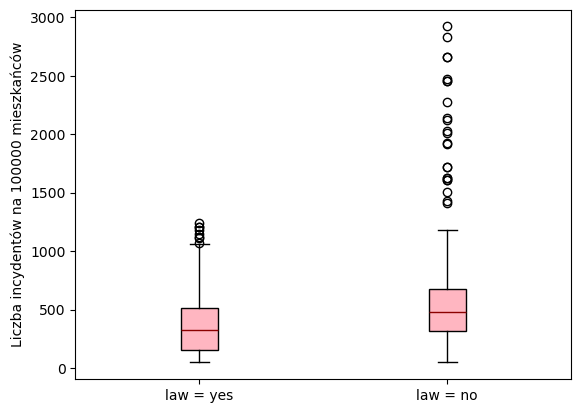
\includegraphics[width=1\textwidth]{img/boxplot.png}
		\caption{Wykresy pudełkowe (boxploty) zmiennej violent dla dwóch grup: z obowiązującym prawem o noszeniu ukrytej broni („law = yes”) oraz bez niego („law = no”).}
		\label{fig:boxplot}
	\end{figure}
	
	Na powyższym wykresie widać, że mediana przestępczości jest znacznie niższa w grupie z prawem. Ponadto rozstęp międzykwartylowy jest tam węższy, a liczba wartości odstających jest mniejsza. W grupie bez prawa widoczny jest długi „ogon” oraz wyższe maksymalne wartości przemocy, co zgadza się z wcześniejszą analizą skośności i kurtozy. Wnioskujemy zatem, że wprowadzenie regulacji prawnych zmniejsza zarówno poziom, jak i ekstremalność przemocy. Zgadza się to z przeprowadzoną wcześniej analizą statystyczną. 
	
	\subsection{Histogram}
	\begin{figure}[H]
		\centering
		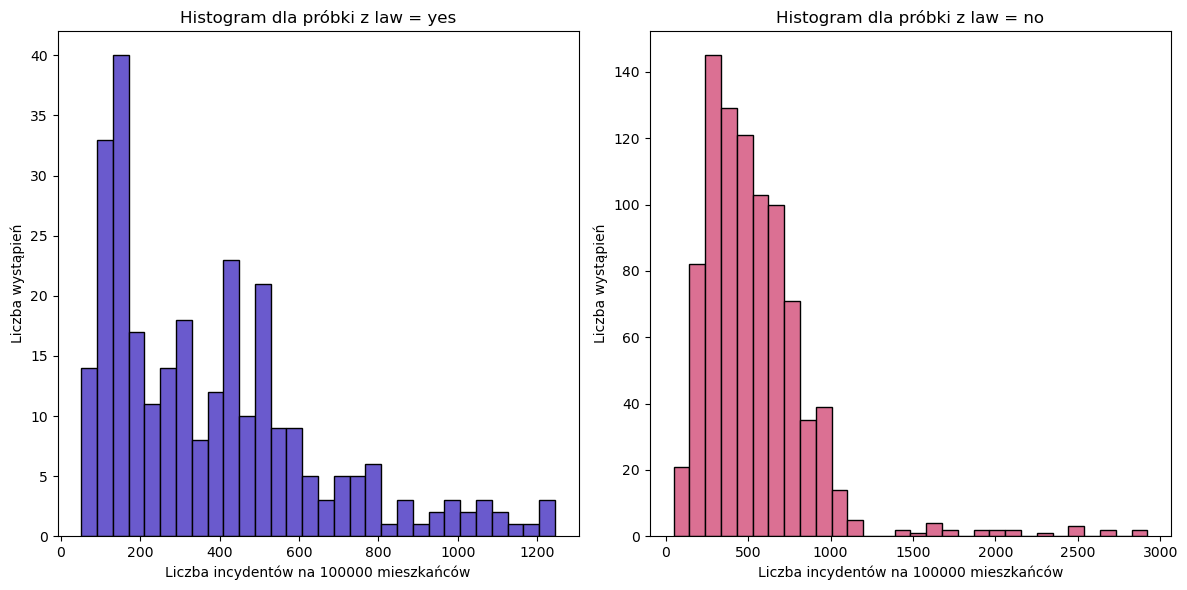
\includegraphics[width=1\textwidth]{img/histogram.png}
		\caption{Histogramy zmiennej violent oddzielnie dla stanów z obowiązującym prawem o noszeniu ukrytej broni („law = yes”) i bez niego („law = no”).}
		\label{fig:histogram}
	\end{figure}
	
	Z wykresu wyraźnie wynika, że w stanach z prawem najwięcej obserwacji przypada na przedziały z niższą liczbą przestępstw, rozkład jest bardziej skupiony wokół wartości do około 400. Natomiast w grupie bez prawa histogram przesuwa się w stronę wyższych wartości: więcej stanów odnotowuje przestępczość na poziomie około 500 przypadków na 100 000 mieszkańców. Patrząc na osie wykresów widzimy znaczną różnicę: oś x-ów próbki z prawem mieści się w zakresie od 0 do 1200, a próbki bez prawa idzie od 0 do aż 3000. Y-kowe osie tych wykresów także znacznie się różnią, na fioletowym wykresie widzimy wartości tylko do 40, a na różowym do 140. Taka różnica w kształcie histogramów potwierdza wyniki wcześniejszej analizy statystycznej. W stanach bez regulacji przemoc była nie tylko wyższa średnio, ale również częstsza w wyższych zakresach, co może wskazywać na większe ryzyko społeczne w tej grupie.
	
	\subsection{Dystrybuanta empiryczna}
	\begin{figure}[H]
		\centering
		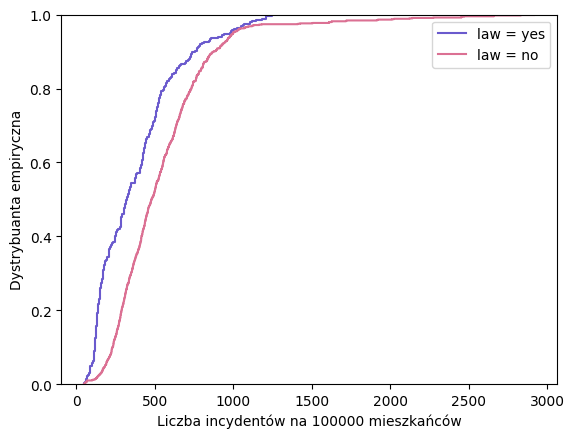
\includegraphics[width=0.8\textwidth]{img/dystrybuanta.png}
		\caption{Dystrybuanta empiryczna zmiennej violent dla stanów z obowiązującym prawem o noszeniu ukrytej broni („law = yes”) i bez niego („law = no”).}
		\label{fig:dystrybuanta}
	\end{figure}
	
	Na wykresie widać wyraźne przesunięcie krzywych dystrybuanty empirycznej: krzywa dla grupy z prawe rośnie szybciej i osiąga wartości bliskie 1 przy niższych poziomach przemocy (ok. 800). Wskazuje to, że większość obserwacji w tej grupie znajduje się w niższych przedziałach liczby przestępstw. Natomiast w próbce bez prawa wzrost krzywej jest wolniejszy --- oznacza to, że wyższe wartości przestępczości występują tam częściej i rozkład jest bardziej rozciągnięty. Wnioski te są spójne z wcześniejszą analizą kwartylową oraz histogramem --- rozkład w grupie bez prawa ma większy rozstęp, skośność i kurtozę, co skutkuje wolniejszym narastaniem dystrybuanty i obecnością wartości ekstremalnych.
	
% kukuplot - chyba nie robimy ale jeszcze zostawie
%	\begin{figure}[H]
%		\centering
%		\includegraphics[width=0.6\textheight]{kuku.png}
%		\caption{Wykresy kwantylowe (QQ plot) dla zmiennej violent osobno dla stanów z obowiązującym prawem dotyczącym noszenia ukrytej broni palnej („law = yes”) oraz bez niego („law = no”).}
%		\label{fig:wykres3}
%	\end{figure}
	
%	W przypadku grupy z prawem punkty układają się stosunkowo blisko czerwonej linii odniesienia, co sugeruje, że dane nie odbiegają drastycznie od rozkładu normalnego – choć w górnym ogonie widoczna jest lekka asymetria. Natomiast dla stanów bez prawa widoczny jest wyraźny odchył od linii prostoliniowej – punkty w górnej części wykresu znacząco odbiegają od linii, co oznacza obecność licznych wartości ekstremalnie wysokich, niespełniających założeń normalności. Wynik ten dobrze koresponduje z wcześniejszą analizą kurtozy i skośności, gdzie wykazano, że rozkład danych w tej grupie był silnie prawoskośny i bardziej „spiczasty”. QQ plot potwierdza zatem, że dane w grupie „law = no” wykazują większe odstępstwa od normalności niż dane z grupy „law = yes”.
	
	\newpage
	{\small \section{Podsumowanie}}
	Przeprowadziliśmy rozległą analizę porównawczą danych dotyczących przestępczości w stanach z i bez prawa "shall carry law", czyli przepisem dotyczącym noszenia ukrytej broni palnej. Wszystkie obliczone miary położenia wyszły wyższe w grupie danych bez tego prawa. Tak samo wyszedł rozstęp, wariancja oraz odchylenie. Rozstęp międzykwartylowy wyszedł nam podobny w obu próbkach. Interesująco, współczynnik zmienności wyszedł trochę większy dla danych z prawem, co oznacza większe rozproszenie względem średniej w tej grupie. Miary kształtu rozkładu wyszły w obu przypadkach większe dla próbki bez obowiązującego prawa. Wyliczone przez nas miary zostały zobrazowane na trzech wykresach --- boxplocie, histogramie i dystrybuancie empirycznej. 
	Uzyskane wyniki wyraźnie pokazują, że wprowadzenie "shall carry law" wiąże się z wyraźnie niższym poziomem przestępstw z użyciem przemocy oraz znacznie mniejszym ryzykiem na występowanie skrajnych, niebezpiecznych sytuacji, jakimi na przykład mogą być strzelaniny.


% ===== WZÓR NA LISTY ====
%	{\small \section{Lista}}
%	\begin{itemize}[itemsep=5pt,parsep=0pt]
%		\item Rzecz 1
%	\end{itemize}
	
	
% ===== WZÓR NA TABELE =====
	
%	\begin{table}[H]
%		\centering
%		\begin{tabular}{|l|c|c|c|}
%			\hline
%			\multicolumn{1}{|c|}{Lp.} & & & \\ \cline{1-3}\hline
%		\end{tabular}\\[0.5cm]
%		\caption{Opis tabeli.}
%		\label{tab1} 
%	\end{table}
	
	
% ===== WZÓR NA RYSUNKI =====

%	\begin{figure}[H]
%		\centering
%		\includegraphics[width=0.97\textheight, angle=90]{plik.pdf}
%		\caption{Opis wykresu.}
%		\label{fig:wykres}
%	\end{figure}

% ===== WZÓR NA OBLICZENIA ====

%	\begin{equation}
%		\begin{aligned}
%			Obliczenia przykładowe.
%		\end{aligned}
%	\end{equation}\\
	
\end{document}